\scanpage{185}
\mspage{95}
% L01–06
ait
\[
\{\deleted{\unsure{s}}\lambda s_0,\lambda^{-1}t_0\}\in A_0\tag*{(17'')}
\]
où $(s_0,t_0)$ est une arête orientée fixée. Cela signifie aussi qu'il existe $g\in G_0$ tel qu'on ait
\[
g(s_0,t_0)=\{\lambda s_0,\lambda^{-1}t_0\}
\]

% L07–12
ou encore, en posant
\[
t_0=\rho(s_0)\qquad\text{pour }\rho\in G_0\text{ convenable}\tag*{(19)}
\]
qu'on ait
\[
\begin{aligned}
&\deleted{\lambda^{-1}us_0=s_0}\\
&g^{-1}\lambda s_0=s_0\qquad
\underbrace{(g\rho)^{-1}\underbrace{\lambda^{-1}\rho}_{\rho\lambda^{-1}}s_0}_{\rho^{-1}g^{-1}\rho\lambda^{-1}s_0}=s_0
\end{aligned}
\]
soit
\[
\exists g\in G_0\deleted{\unsure{\in}}\quad\text{tel que}\quad g^{-1}\lambda s_0=s_0,\quad\rho^{-1}(g^{-1})\lambda^{-1}s_0=s_0.\tag*{(20)}
\]

% L13–16
Explicitant alors $\lambda$ à l'aide d'un élément
\[
a\in\operatorname{Norm}_{G_0}(\widetilde U)\qquad\lambda s_0=as_0\deleted{\unsure{\in}}\tag*{(21)}
\]
% slanted
\margin{Je pose maintenant $\widetilde U=G_{0s_0}$ réservant la notation $U$ à $G^+_{0\,s_0}$ (quand il y a un $G_0^+$ \unsure{--})}
la condition (20) s'écrit
\[
\exists g\in G_0\quad\text{tel que}\quad g^{-1}a\in\widetilde U,\quad\rho^{-1}(g^{-1})a^{-1}\in\widetilde U\tag*{(22)}
\]

% L17–19
où on \deleted{peut} prend pour $\rho$ un quelconque élément satisfaisant (19) (déterminé mod $U$ i.e. pft\textsuperscript{ment} déterminé) p.ex. on peut prendre
\[
\rho=\deleted{\unsure{g}}\tau_0,\ \text{ou } \underset{\substack{\shortparallel\\\tau_0\tau_\infty\\\shortparallel\\\tau_\infty\tau_0}}{\unsure{\lambda_1|\rho_1}},\
\text{ou }\underset{\substack{\shortparallel\\\tau_0\tau_1}}{\unsure{\lambda_\infty^{-1}|\rho_\infty^{-1}}}=\rho,\quad\text{au choix}.\tag*{(23)}
\]
\margin{les $\rho$ du formulaire pour $\mathrm{SL}(2,Z)$\ldots}
\figure{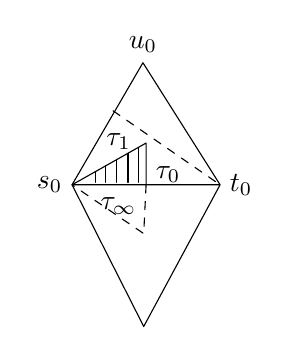
\begin{tikzpicture}[x=1cm,y=1cm,line cap=round,line join=round]
\draw (0,0)--(.9,1.55) node[above]{$u_0$} --(1.88,0) node[right]{$t_0$}--(.91,-1.8)--(0,0) node[left]{$s_0$}--(1.88,0);
\draw[dashed] (.52,.94)--(1.88,0);
\draw (0,0)--(.94,.53)--(.94,0);
\draw[dashed] (.94,0)--(.91,-.62)--(0,0);
\foreach \x in {.30,.43,.57,.71,.84}{\draw (\x,.03)--(\x,{.53*\x/.94});}
\node at (.59,.55){$\tau_1$};\node at (1.22,.13){$\tau_0$};\node at (.59,-.27){$\tau_\infty$};
\end{tikzpicture}}

% L20–22
La relation 22 s'écrit aussi, posant $g^{-1}a=u$
\[
\exists u\in U\quad\text{tel que}\quad\rho^{-1}(ua^{-1})a^{-1}\in\widetilde U\qquad\text{i.e.}\tag*{\deleted{(22)}}
\]
\[
\begin{aligned}
&\text{i.e. }\rho(a)a\in\unsure{\rho(\widetilde U).u|{\rho(\widetilde U).U}} \qquad
a\,\rho^{-1}(au^{-1})\in\widetilde U\quad\text{i.e. }a\,\rho^{-1}(a)\in\widetilde U\,\rho^{-1}(u),\\
&\hspace{9em}\deleted{\text{i.e. }\rho(a)a\in\rho(\widetilde U)U}
\end{aligned}
\]

% archive sheet number: 184
